\section*{Section A}
\label{sec:Section A}
\FloatBarrier % Now figures cannot float above section title


In this section, the Young's modulus of two materials 
(mild steel and aluminium) can be calculated from experimental data.

A total of six groups of data were obtained from the experiment. (See Table \ref{t1})


\subsection*{Analysis}

By plotting these 6 groups of data on a scatter plot and performing 
regression analysis, a total of 6 groups of graphs were obtained.

\begin{figure}
    \centering
    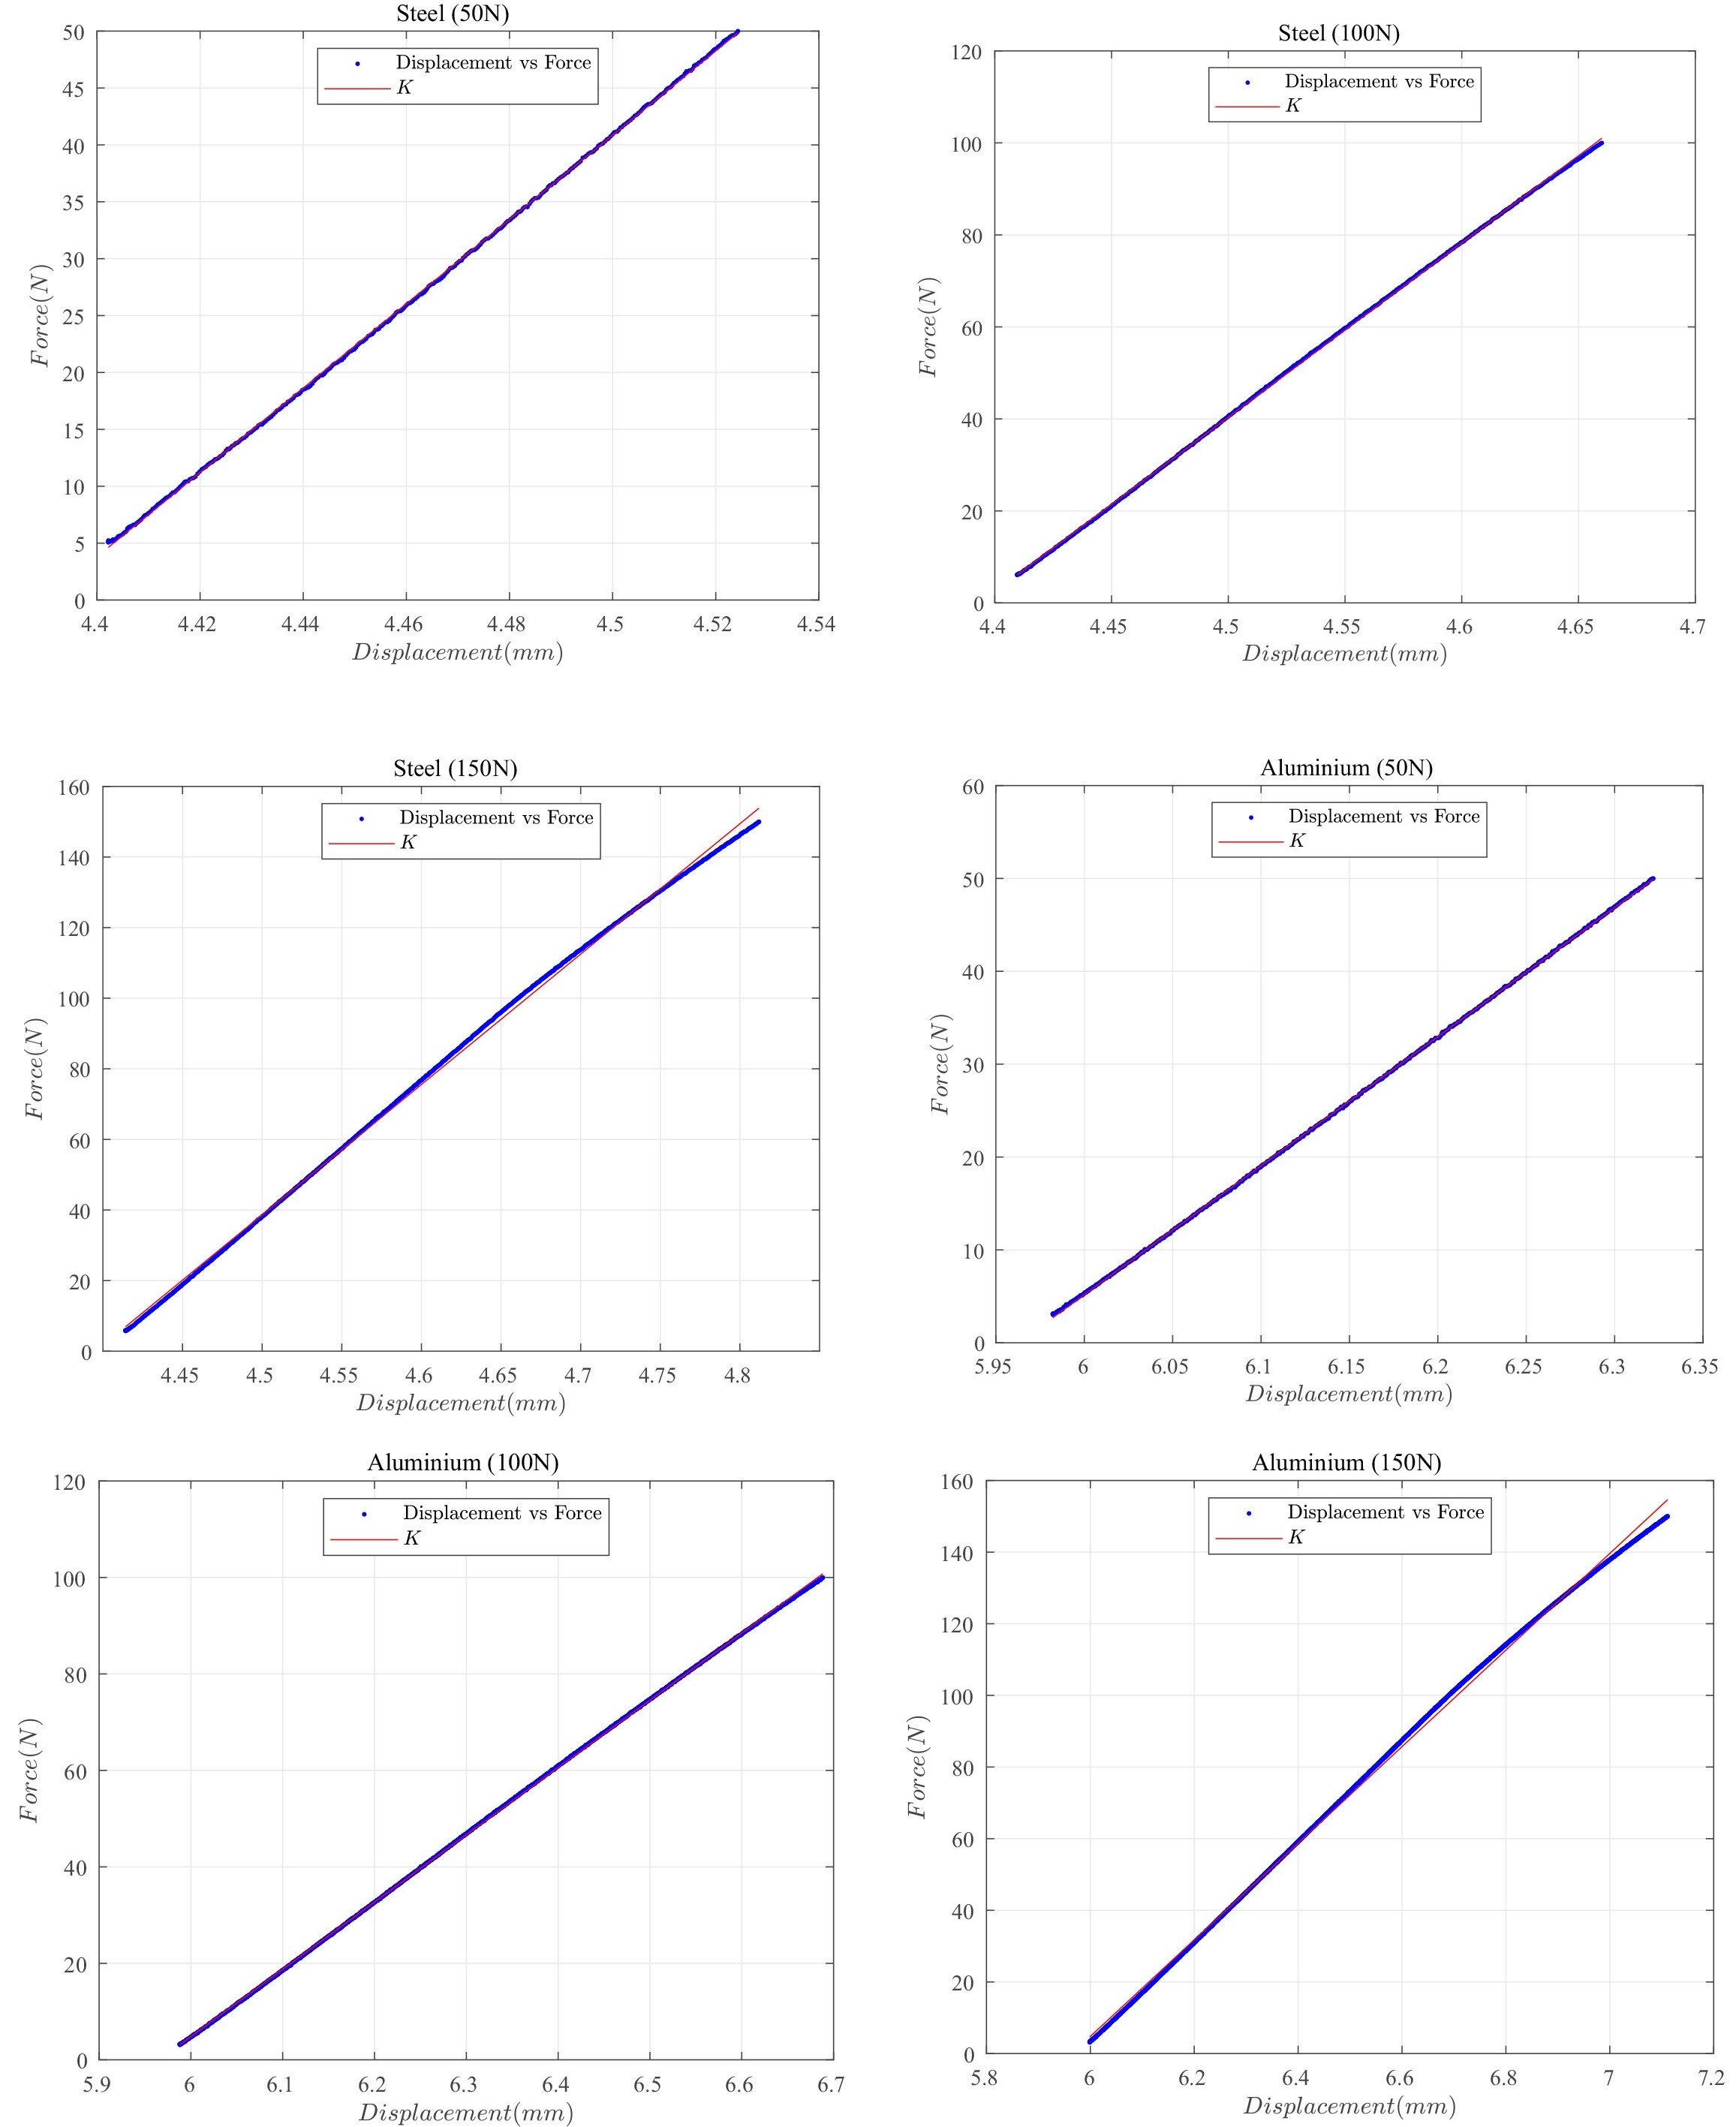
\includegraphics[width=18.7cm,height=26cm]{./fig/mix.jpg}
    \caption{This is an inserted JPG graphic}
    \label{f1}
\end{figure}

\begin{minipage}[t]{\textwidth}
    \makeatletter\def\@captype{table}
    \centering
    \scalebox{1.1}{
    \begin{tabular}{llll} 
        \hline
        No.  & Material    & Final load (N) & R-square    \\ \hline
        1 & Steel     & 50   & 0.9999\\
        2 & Steel      & 100  & 0.9998\\
        3 & Steel      & 150   & 0.9989\\
        4 & Aluminium     & 50  & 0.9999\\
        5 & Aluminium    & 100   & 0.9999\\
        6 & Aluminium & 150   & 0.9987\\ \hline          
    \end{tabular}} 
    \caption{result of A1 regression analysis}
    \label{t1} 
\end{minipage}

In order to calculate E, the moment of inertia I needs to be calculated first.

\begin{equation} 
I=\frac{bh^3}{12}=\frac{20*3^3}{12}*10^{-12}=4.5*10^{-11} (mm^4)
\end{equation}

We know 
\begin{equation} 
    \delta_{max}=\frac{PL^3}{48EI}
\end{equation}

And the slope of the regression analysis
\begin{equation} 
    K=\frac{P}{\delta}=\frac{48EI}{L^3}
\end{equation}

So

\begin{equation} 
    E=(\frac{P}{\delta})*\frac{L^3}{48}=K*\frac{L^3}{48}
\end{equation}

\begin{minipage}[t]{\textwidth}
    \makeatletter\def\@captype{table}
    \centering
    \scalebox{1.1}{
    \begin{tabular}{lll} 
        \hline
        Modulus of Elasticity  & Mild Steel    & Aluminium     \\ \hline
        $E_1(P=50N)$ & 171.482     & 64.3056    \\
        $E_2(P=50N)$ & 175.509     & 64.5370   \\
        $E_3(P=50N)$ & 171.019     & 62.4074   \\
        $E_{exp}=(E_1+E_2+E_3)/3$ & 172.670 & 63.75   \\ \hline          
    \end{tabular}} 
    
    (Unit: GPa)
    \caption{result of A1 regression analysis}
    \label{table4} 
\end{minipage}


\subsection*{Summary}



